\chapter{User Testing and Feedback Summary}
\label{chap:feedback}

\section{Purpose}

The purpose of our user testing was to determine which of our two mockups ---
the red line/transition lens glasses and the vibrating arm cuff --- would
provide a more effective stimulus for drawing the user’s attention to their
left side. In addition, we were looking for user insights into the comfort and
usability of our designs.

\section{Methodology}

One team member conducted one user test session, at Alexian Brothers
Rehabilitation Hospital under the supervision of Dr. Kate Enzler, with our
mockups during the week of February 6th. The mockups were a pair of glasses
with interchangeable velcro attachments to simulate different visual stimuli
and an adjustable arm band containing a haptic motor. The mockups differed
mainly in the stimuli being used to draw attention to the left side. Below are
photos of the mockups used during the testing. \autoref{fig:glasses} shows the
glasses with various attachments and \autoref{fig:strap} shows the vibrating
arm band.

\begin{figure}[h]
  \centering
  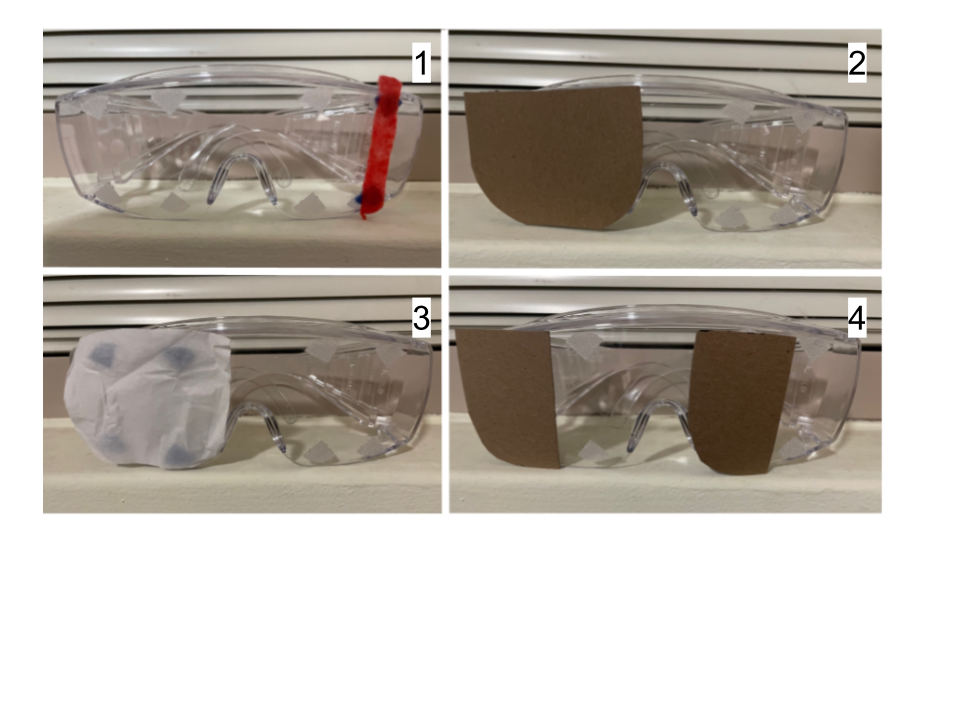
\includegraphics[width=0.75\textwidth]{glasses}
  \caption[Design 1: Glasses and Attachments]{Glasses with various attachments
    (attachment 1: red felt line, attachment 2: opaque patch, attachment 3:
    transparent patch, attachment 4: opaque half patches).}
  \label{fig:glasses}
\end{figure}

\begin{figure}[h]
  \centering
  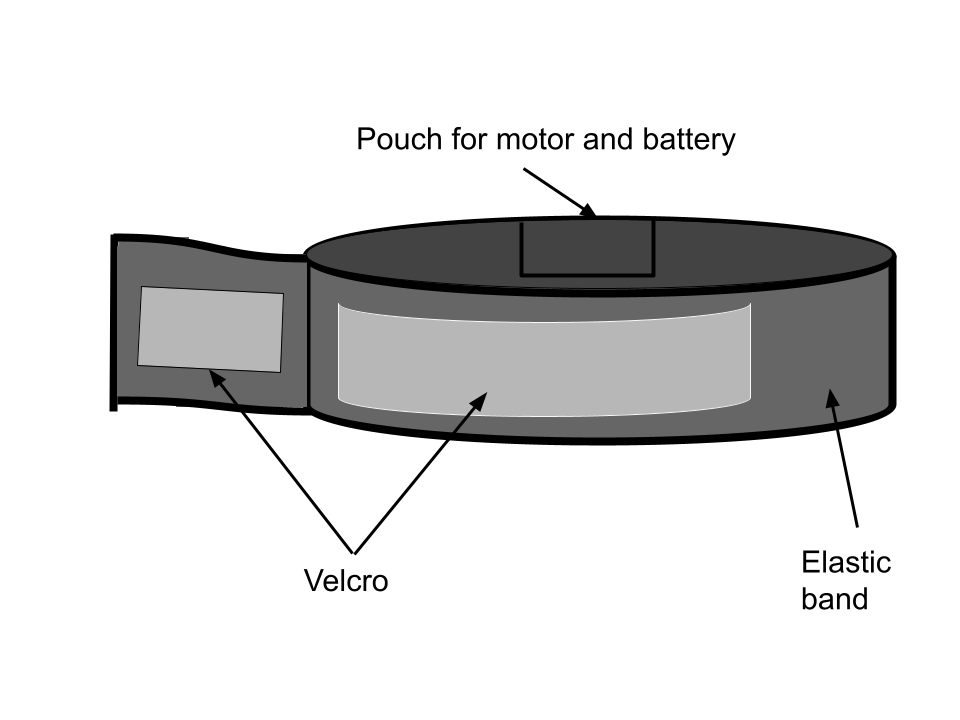
\includegraphics[width=0.75\textwidth]{strap}
  \caption[Design 2: Arm-band]{Arm-band haptic feedback mockup.}
  \label{fig:strap}
\end{figure}

During the user testing session, the user was asked to try on each mockup one
at a time.  A team member stood to the left side of the user and held up a
number with their fingers, observing if the user turned their head towards the
team member due to the stimuli from the mockup. After, the user was asked if
they saw the number the team member was holding up. Then, the user was asked to
provide feedback on how effective the design was at drawing attention to their
left side and on how comfortable the design would be for daily wear.

\section{Results}

\subsection{Glasses}

When the user put on the glasses, they were able to see the red line, but it
did not cause them to turn their head. They stated that it would take them a
while to know whether it would work or not. When the line was moved closer to
the eye, the user found it too close to their field of vision to be
comfortable. However, it should be noted that another team tested how a pair of
glasses of similar design improved the user’s ability to read, and that design
helped the user identify almost all of the letters on a page.

\subsection{Arm Band}

When the arm band mock-up was introduced, Dr. Enzler showed the team members
present that the user had no feeling in their left arm by touching the arm and
confirming with the user that they could not feel it. So, the mock-up was not
used as intended; instead, it was placed around the user’s head so that the
vibration was near the user’s ear. The user stated that the vibration was very
noticeable, and it caused the user to turn their head far enough that they were
able to accurately read the number that a team member was holding up.

\section{Analysis, Conclusions and Limitations}

\subsection{Analysis of Results}

\subsubsection{Glasses}

The user did not find this mockup to be particularly effective at first use,
stating that they would need about a month of wearing it to truly know if it
was effective or not. It seems that because the visual cue would be moving with
the user’s head, it might not be as effective as a visual cue that remains
stationary and serves as a basis for where the user should turn their attention
to.

\subsubsection{Arm Cuff}

The original placement for this idea didn’t work as intended because the user
had very limited feeling on the left side of the body below the neck. But, when
repositioning the mockup to be used as a headband so it vibrated around the
user’s ear, it seemed to be the one of the most effective stimuli of the
testing session, as the user immediately turned their head and was able to see
the number that the team member was holding up.

\subsection{Conclusion}

The results suggest that haptic stimuli around the head can be an effective
method for drawing attention to the left side. The arm band design can be
repurposed as a vibrating accessory worn around the head, and can be improved
by incorporating the capability of tracking how far the user has turned their
head after receiving the stimuli. In addition, the results suggest that the
glasses design was not effective in the use it was intended for, but results
from other teams indicate that there are certain scenarios like reading where
this pair of glasses might have value. One main takeaway from the testing
session is that different designs can be effective in specific scenarios, so it
may be worthwhile to explore how each team might make a design that plays a
certain role in the larger whole of left-neglect rehabilitation.

\subsection{Limitation}

One of the largest limitations of this test session was the sample size of only
one user. While the user provided important insights, it is also known that
left neglect treatment is often customized and different solutions work best
for different people, so it would have been helpful to test the mockups with
more than one user. However, this limitation is one that is difficult to
remediate due to the fact that Dr. Enzler only has a limited number of patients
who would be able to participate in testing.

Another limitation to our testing methodology was that our design ideas
incorporated electronics, but the mockups did not have independently working
electronics. Since the functionality of our designs depends largely on these
electronics, we were not able to thoroughly test the usability of designs. This
limitation was especially prominent in the glasses mock-up, as ideally the
visual stimuli would be turning on and off but since the attachments were
static, it was hard to know if they would truly grab a user’s attention or
not.


%%% Local Variables:
%%% mode: latex
%%% TeX-master: "../final_report"
%%% End:

